\section{Updating the Game State}

\subsection{Raw State Information}

The ORTS API provides complete game state update information in the form
of 6 lists:

\begin{itemize}
  \item \verb|new_tile_indexes| New game tiles encountered via
  uncovering of fog of war.
  \item \verb|new_objs| New game objects, such as enemy units and
  buildings, or world objects such as trees.
  \item \verb|changed_objs| Game objects that have changed since the
  previous viewframe.
  \item \verb|vanished_objs| Game objects that disappeared from the
  player's vision.
  \item \verb|dead_objs| Game objects that died.
  \item \verb|new_boundaries| New terrain boundaries that demarcate
  the border between different terrain types, such as ground and cliff.
\end{itemize}

SORTS currently takes into account the information in all
the lists except \verb|new_tile_indexes| and
\verb|new_boundaries|. The former is ignored because SORTS
currently does not have any functioning capability to reason about
terrain, except for collision detection. The latter is ignored because
we get this information from the game tiles directly whenever we check
for boundaries. Note also that currently, SORTS treats objects vanishing
(reported in \verb|vanished_objs|) and objects dying (reported in
\verb|dead_objs|) as one and the same thing. This will probably change
in the future as agents use more sophisticated reasoning.

All game state updates, both internal to the middleware and to the Soar
input link, are performed in the ORTS event handler, which is triggered
everytime the middleware receives a new viewframe from the ORTS server.
An overview of the flow of control among the various functions is shown
in figure~\ref{fig:flow}. Detailed descriptions of the two event
handlers are provided below.

\begin{figure}
\includegraphics[width=\textwidth]{graphics/flow.eps}
\caption{Overview of how control is passed through Sorts. Note that the
two gray regions represent two different threads executing
asynchronously.}
\label{fig:flow}
\end{figure}

\subsection{The ORTS Event Handler}
\label{sec:OrtsEventHandler}

The ORTS event handler is triggered everytime the middleware receives
a new viewframe from the ORTS server. This event handler and the
Soar event handler are the main functions from which most other
function calls are made. Pseudo-code for the handler is shown in
figure~\ref{fig:OrtsEventHandler}.

\begin{figure}
\begin{verbatim}
ORTSEventHandler
  lockMutex()
  mergeChanges(oldChanges, changes)
  if currentViewFrame - lastActionFrame > ALLOWED_LAG then
    unlockMutex()
    return
  end
  removeDeadObjects(changes)
  assignSoarActions()
  updateSoarGameObjects(changes)
  sendActions()
  updateGroups()
  unlockMutex()
end
\end{verbatim}
\caption{Pseudo code for the ORTS event handler}
\label{fig:OrtsEventHandler}
\end{figure}

Each function call is described below.

\begin{itemize}

\item \verb|lockMutex()| and \verb|unlockMutex()|
  This mutex locks the Soar event handler from executing until the
  ORTS event handler is finished. This is important since we don't want
  the Soar command buffer to change while we are processing that buffer.

\item \verb|mergeChanges(oldChanges, changes)|
  If SORTS falls behind the ORTS server too much, changes to the game
  state will be accumulated but not processed in the interest of
  catching up. This function merges changes reported in previous
  viewframes with the current changes.

\item \verb|removeDeadObjects(changes)|
  This function removes all game objects that have just died or vanished
  in the current frame. This call needs to be made before the call to
  \verb|assignSoarActions()| so that we don't try to assign any actions
  to objects that disappeared, which the ORTS server would not
  understand.

\item \verb|assignSoarActions()|
  Interprets commands queued from the Soar output-link as ORTS actions and
  distributes them to the appropriate groups. The actions are not sent
  to the ORTS server until \verb|sendActions()| is called.

\item \verb|updateSoarGameObjects(changes)|
  This is the main function that updates the attributes of the
  SoarGameObject structures in the middleware. It is called after
  \verb|assignSoarActions()| so that units will begin responding to
  their commands in the Soar cycle that immediately follows the one in
  which they were assigned.

\item \verb|sendActions()|
  This is a call to the ORTS API that sends all queued actions to the
  server.

\item \verb|updateGroups()|
  Runs the grouping algorithm over SoarGameObjects that have changed or
  appeared, and prunes those groups whose members have died. These
  changes are directly reflected in the Soar input-link, but are
  buffered in the SML interface until the next Soar decision cycle.

\end{itemize}

\subsection{The Soar Event Handler}
\label{sec:SoarEventHandler}

The Soar event handler is triggered at the end of each Soar decision
cycle. The main responsibility of this function is to take commands off
the Soar output-link and buffer them into action queues in the
middleware.

\begin{figure}
\begin{verbatim}
SoarEventHandler
  lockMutex()
  if Catchup = true then
    unlockMutex()
    return
  end if
  getNewSoarOutput()
  processVisionCommands()
  processGameCommands()
  unlockMutex()
end
\end{verbatim}
\caption{Pseudo code for the Soar event handler}
\label{fig:SoarEventHandler}
\end{figure}

Figure~\ref{fig:SoarEventHandler} shows the pseudo-code for the
function. The following is a list of descriptions for each call made in
the function.

\begin{itemize}

\item \verb|lockMutex()| and \verb|unlockMutex()|
  These calls lock on the same mutex as the ORTS event handler, thereby
  making the execution of these two functions mutually exclusive.

\item \verb|getNewSoarOutput()|
  Takes all commands on the Soar output-link and queues them into lists
  in the middleware. This includes both commands issued to in-game units
  as well as commands that adjust middleware parameters such as grouping
  radius and center of visual attention. However, none of the commands
  are actually processed by this function.

\item \verb|processVisionCommands()|
  Processes Soar commands related to the perceptual system. These
  commands include changing the grouping radius, looking at a specific
  coordinate, looking at a feature in the feature map, and changing the
  maximum number of objects allowed on the input-link at any time (for
  a complete list, see section~\ref{sec:output-link}. These commands
  are processed here rather than with the in-game commands because Soar decision cycles can occur much faster than ORTS events.

\item \verb|processGameCommands()|
  Handles all commands that affect the way the middleware executes
  low-level actions, such as in the FSMs, but do not translate directly
  into ORTS game object actions. Also handles miscellaneous queries that
  Soar may make to the middleware for information not normally provided
  to it. Currently, there are only three such commands: finding a
  location for a building, and setting and clearing the mineral buffer
  (see section~\ref{sec:output-link}).

\end{itemize}
